\documentclass{standalone}
\usepackage{tikz}
\usepackage{tikz-network}
\usepackage{subcaption}
\usepackage{graphicx}
% \usetikzlibrary{graphs, graphdrawing, positioning, quotes}
\usepackage{color}
\definecolor{lightblue}{RGB}{158,202,225}
\begin{document}
    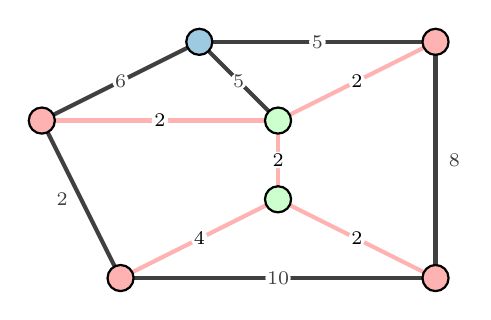
\begin{tikzpicture}
        \coordinate (v1) at (0,0);
        \coordinate (v2) at (3,0);
        \coordinate (v3) at (1,-1);
        \coordinate (v4) at (-2,-1);
		\coordinate (v5) at (-1,-3);
		\coordinate (v6) at (1,-2);
		\coordinate (v7) at (3,-3);

        \node[draw,circle,fill=lightblue,thick,minimum size=8pt] (CircleNode) at (v1){};
		\node[draw,circle,fill=red!30,thick,minimum size=8pt] (CircleNode) at (v2){};
		\node[draw,circle,fill=green!20,thick,minimum size=8pt] (CircleNode) at (v3){};
		\node[draw,circle,fill=red!30,thick,minimum size=8pt] (CircleNode) at (v4){};
		\node[draw,circle,fill=red!30,thick,minimum size=8pt] (CircleNode) at (v5){};
		\node[draw,circle,fill=green!20,thick,minimum size=8pt] (CircleNode) at (v6){};
        \node[draw,circle,fill=red!30,thick,minimum size=8pt] (CircleNode) at (v7){};

        \Edge[label=$5$](v1)(v2)
        \Edge[label=$5$](v1)(v3)
        \Edge[label=$6$](v1)(v4)
        \Edge[label=$2$,color=red!30,fontcolor=black](v2)(v3)
        \Edge[label=$2$,position={left=1mm}](v4)(v5)
        \Edge[label=$2$,color=red!30,fontcolor=black](v4)(v3)
        \Edge[label=$2$,color=red!30,fontcolor=black](v3)(v6)
        \Edge[label=$4$,color=red!30,fontcolor=black](v5)(v6)
        \Edge[label=$10$](v5)(v7)
        \Edge[label=$8$,position={right=1mm}](v2)(v7)
        \Edge[label=$2$,color=red!30,fontcolor=black,](v6)(v7)    
    \end{tikzpicture}
\end{document}